\begin{homeworkProblem}

\textbf{Beta Normal Distribution:} generate samples from the beta distribution $\Beta(5,5)$

(a) Implement a Metropolis-Hastings algorithm.

(b) Implement a Hamiltonian Monte Carlo algorithm.

(c) Implement with the Acceptance-Rejection Method.

(d) Compare the above three algorithms with corresponding pros and cons.

\solution

Let $X\sim \Beta(5,5)$. We can calculate the beta integral:
$$\beta(5,5)=\dfrac{\Gamma(5)\cdot\Gamma(5)}{\Gamma(10)}=\dfrac{4!\cdot 4!}{9!}=\dfrac{1}{630}$$
Then we can calculate the PDF of $X$:
$$f(x)=f_X(x)=\dfrac{1}{\beta(5,5)}x^{5-1}(1-x)^{5-1}=630x^4(1-x)^4 ,0<x<1$$

(a) Since the support of Beta distributio is $[0,1]$, so we can choose the proposal distribution to be $\Unif(1)$, which means that the one-step transition probability density from state $x$ to $y$ is $f_{x,y}=1$, thus we can get that the acceptance rate:
$$a_{x,y}=\min\left(\dfrac{\pi_jf_{j,i}}{\pi_if_{i,j}},1\right)=\min\left(\dfrac{j^4(1-j)^4}{i^4(1-i)^4},1\right)$$
Then we can do the Discrete time continuous state Metropolis-Hastings algorithm to sample the distribution $\Beta(5,5)$ in 1000000 samples, and the burn in is set to be 10000 samples. The result is as follows:
\begin{figure}[h]
    \centering
    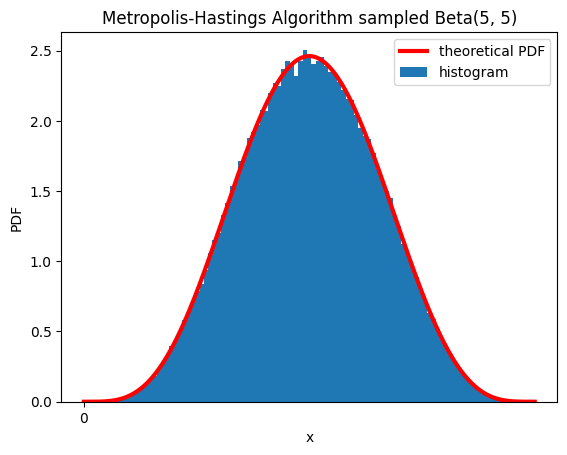
\includegraphics[width=0.5\textwidth]{./figure/p5/MH.png}
\end{figure}

(b) Since $\pi_x$ is a the stationary distribution $\Beta(5,5)$, and we can ignore the constant form, so the potential energy is
$$U(x)=-\log(\pi_x) = -\log(630) -4\log(x(1-x)) \stackrel{\text{ignore const}}{\Rightarrow} U(x)=-4\log(x(1-x))$$
And let the mass be 1, then the Kinetic energy is
$$V(\omega)=\dfrac{1}{2}\omega^2, \quad\text{where } \omega\sim\N(0,1)$$
Thus the Hamiltonian energy is
$$H(x,\omega)=U(x)+V(\omega)=-4\log(x(1-x))+\dfrac{1}{2}\omega^2$$
Initially, set $x_0=0.5, \omega_0\sim\N(0,1)$, apply the Leapfrog method to sample:
\begin{align*}
\omega_{t+\frac{\delta}{2}} &= \omega_t - \frac{\delta}{2}\cdot \dfrac{\dU(x_t)}{\dx_t} = \omega_t - \frac{\delta}{2}\cdot \left(-\dfrac{4}{x_t}+\dfrac{4}{1-x_t}\right) \\
x_{t+\delta} &= x_t + \delta \cdot \dfrac{\dV(\omega_{t+\frac{\delta}{2}})}{\domega_{t+\frac{\delta}{2}}} = x_t + \delta\cdot \omega_{t+\frac{\delta}{2}} \\
\omega_{t+\delta} &= \omega_{t+\frac{\delta}{2}} - \frac{\delta}{2}\cdot \dfrac{\dU(x_{t+\delta})}{\dx_{t+\delta}} = \omega_{t+\frac{\delta}{2}} - \frac{\delta}{2}\cdot \left(-\dfrac{4}{x_{t+\delta}}+\dfrac{4}{1-x_{t+\delta}}\right)
\end{align*}
Due to the range limitation of $x\in(0,1)$, we can add a reflection bound at $x=0$ and $x=1$, i.e. when applying Leapfrog, if $x<0$, then set $x\gets -x, \omega\gets -\omega$, if $x>1$, then set $x\gets 2-x, \omega\gets -\omega$. After Leapfrog $L$ steps, we can get the state $(x_L, \omega_L)$. And set $(x_L, -\omega_L)$ to be the proposal distribution. And the accept rate for the Hamiltonian Monte Carlo algorithm is
$$a_{(x_0,\omega_0),(x_L,-\omega_L)}=\min\left(\dfrac{\exp\left(-H(x_L,-\omega_L)\right)}{\exp\left(-H(x_0,\omega_0)\right)}, 1\right)=\min\left(\dfrac{\exp\left(-U(x_L)-V(-\omega_L)\right)}{\exp\left(-U(x_0)-V(\omega_0)\right)}, 1\right)$$
We step the stepsize to be $\delta=0.05, L=15$, additionally, since the support is $(0,1)$, so for numerical accuracy, we clip x into the range $[10^{-10},1-10^{-10}]$. One trajectory and sample results are as follows:
\begin{figure}[h]
    \centering
    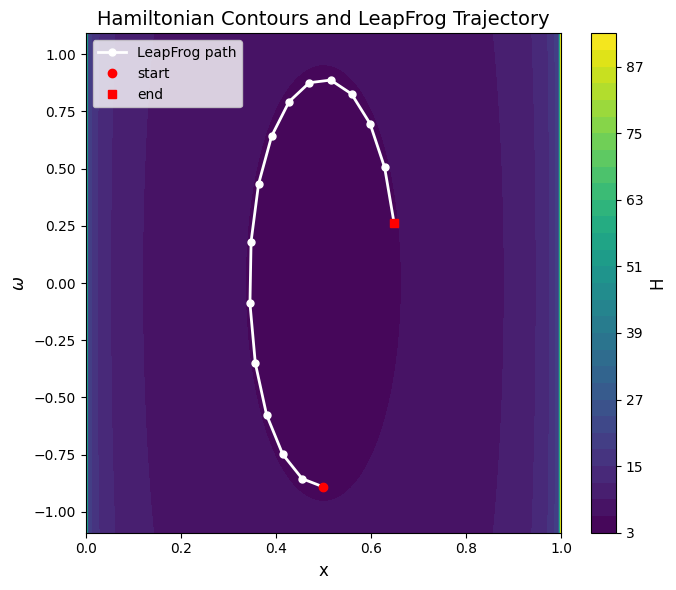
\includegraphics[width=0.5\textwidth]{./figure/p5/trajectory.png}
    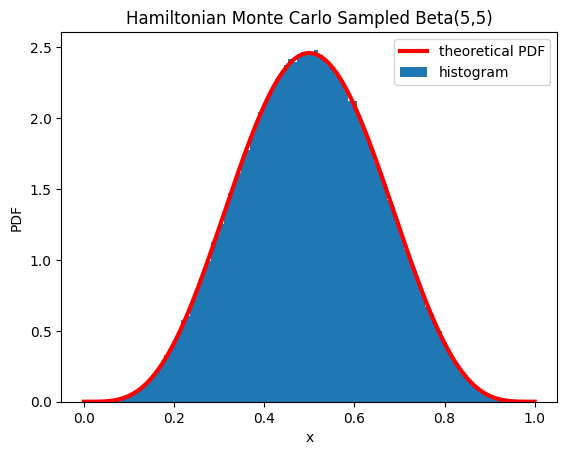
\includegraphics[width=0.5\textwidth]{./figure/p5/Hamiltonian.png}
\end{figure}

(c) As for the acceptance-rejection algorithm, since the support of Beta distribution is $(0,1)$, so we can take $Y\sim \Unif(0,1)$. And its PDF is $g(y)=f_Y(y)=1$. \\
Let $c$ donate a constant:
$$c = \sup_y\dfrac{f(y)}{g(y)} = \sup_y\dfrac{20y(1-y)^3}{1}=630x^4(1-x)^4\big|_{y=\frac{1}{2}}=\dfrac{315}{128}$$
Then we can apply the Acceptance-Rejection algorithm to generate the samples on $X\sim \Beta(5,5)$:
\begin{figure}[h]
    \centering
    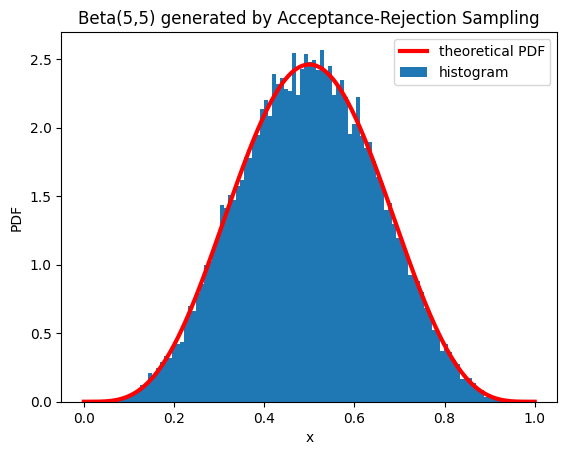
\includegraphics[width=0.5\textwidth]{./figure/p5/accept_reject.png}
\end{figure}

(d) 1. Metropolis-Hastings Algorithm: \\
Advantages: It is highly general-purpose, could applicable to a wide variety of distributions, and it does not require the normalization constant of the target distribution. \\
Disadvantages: Samples are often requires select a suitable distribution, and requires steps to burn up.

2. Hamiltonian Monte Carlo Algorithm: \\
Advantages: Due to the conservation of energy, the acceptance rate should be $1$. But there exists numerical error, however quite close to $1$, which means it has quite high acceptance rate. The samples are efficient, especially in high-dimensional problems. \\
Disadvantages: Requires computation of gradients, increasing implementation complexity. Sensitive to parameters: step size $\delta$ and number of steps for LeapFrog $L$.

3. Acceptance-Rejection Method: \\
Advantages: It produces independent samples, and is simple to implement. If the good envelope function is suitable, it is efficient. \\
Disadvantages: Efficiency depends heavily on the choice of proposal distribution, for example, ours implement has a quite low acceptance rate, which is only 0.0038838.

\end{homeworkProblem}

\newpage